\begin{figure}[th]
    \centering
    \resizebox{0.99\textwidth}{!}{


\tikzset{every picture/.style={line width=0.75pt}} %set default line width to 0.75pt

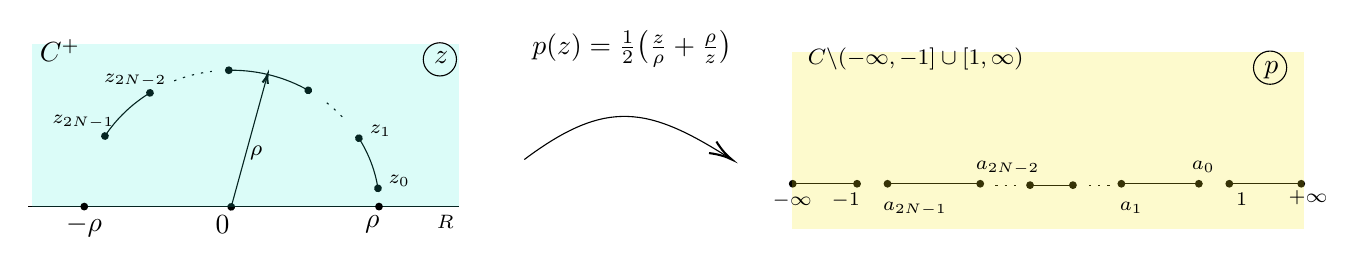
\begin{tikzpicture}[x=0.75pt,y=0.75pt,yscale=-1,xscale=1]
%uncomment if require: \path (0,300); %set diagram left start at 0, and has height of 300

%Straight Lines [id:da11043395115642407]
\draw    (61,166) -- (268.33,166) ;
%Shape: Arc [id:dp5857971438825527]
\draw  [draw opacity=0] (97.96,132.01) .. controls (103.47,123.68) and (110.89,116.57) .. (119.64,111.21) -- (158.8,167.13) -- cycle ; \draw    (97.96,132.01) .. controls (103.47,123.68) and (110.89,116.57) .. (119.64,111.21) ; \draw [shift={(119.64,111.21)}, rotate = 323.47] [color={rgb, 255:red, 0; green, 0; blue, 0 }  ][fill={rgb, 255:red, 0; green, 0; blue, 0 }  ][line width=0.75]      (0, 0) circle [x radius= 1.34, y radius= 1.34]   ; \draw [shift={(97.96,132.01)}, rotate = 308.77] [color={rgb, 255:red, 0; green, 0; blue, 0 }  ][fill={rgb, 255:red, 0; green, 0; blue, 0 }  ][line width=0.75]      (0, 0) circle [x radius= 1.34, y radius= 1.34]   ;
%Shape: Arc [id:dp48308113060202285]
\draw  [draw opacity=0] (157.63,100.31) .. controls (158.02,100.3) and (158.41,100.3) .. (158.8,100.3) .. controls (172.39,100.3) and (185.09,103.84) .. (195.91,109.99) -- (158.8,167.13) -- cycle ; \draw    (157.63,100.31) .. controls (158.02,100.3) and (158.41,100.3) .. (158.8,100.3) .. controls (172.39,100.3) and (185.09,103.84) .. (195.91,109.99) ; \draw [shift={(195.91,109.99)}, rotate = 25.21] [color={rgb, 255:red, 0; green, 0; blue, 0 }  ][fill={rgb, 255:red, 0; green, 0; blue, 0 }  ][line width=0.75]      (0, 0) circle [x radius= 1.34, y radius= 1.34]   ; \draw [shift={(157.63,100.31)}, rotate = 3.52] [color={rgb, 255:red, 0; green, 0; blue, 0 }  ][fill={rgb, 255:red, 0; green, 0; blue, 0 }  ][line width=0.75]      (0, 0) circle [x radius= 1.34, y radius= 1.34]   ;
%Shape: Arc [id:dp5615899707798235]
\draw  [draw opacity=0] (220.31,133.04) .. controls (224.93,140.31) and (228.12,148.48) .. (229.51,157.2) -- (158.8,167.13) -- cycle ; \draw    (220.31,133.04) .. controls (224.93,140.31) and (228.12,148.48) .. (229.51,157.2) ; \draw [shift={(229.51,157.2)}, rotate = 75.29] [color={rgb, 255:red, 0; green, 0; blue, 0 }  ][fill={rgb, 255:red, 0; green, 0; blue, 0 }  ][line width=0.75]      (0, 0) circle [x radius= 1.34, y radius= 1.34]   ; \draw [shift={(220.31,133.04)}, rotate = 62.88] [color={rgb, 255:red, 0; green, 0; blue, 0 }  ][fill={rgb, 255:red, 0; green, 0; blue, 0 }  ][line width=0.75]      (0, 0) circle [x radius= 1.34, y radius= 1.34]   ;
%Shape: Arc [id:dp36745803345523487]
\draw  [draw opacity=0][dash pattern={on 0.84pt off 2.51pt}] (131.32,105.41) .. controls (137.04,103.19) and (143.13,101.63) .. (149.49,100.86) -- (158.8,167.13) -- cycle ; \draw  [dash pattern={on 0.84pt off 2.51pt}] (131.32,105.41) .. controls (137.04,103.19) and (143.13,101.63) .. (149.49,100.86) ;
%Shape: Arc [id:dp11470689402830425]
\draw  [draw opacity=0][dash pattern={on 0.84pt off 2.51pt}] (204.84,116) .. controls (208.03,118.51) and (210.98,121.28) .. (213.66,124.27) -- (158.8,167.13) -- cycle ; \draw  [dash pattern={on 0.84pt off 2.51pt}] (204.84,116) .. controls (208.03,118.51) and (210.98,121.28) .. (213.66,124.27) ;
%Straight Lines [id:da16372735936793958]
\draw    (158.8,166.13) -- (175.8,104.26) ;
\draw [shift={(176.33,102.33)}, rotate = 105.37] [color={rgb, 255:red, 0; green, 0; blue, 0 }  ][line width=0.75]    (4.37,-1.32) .. controls (2.78,-0.56) and (1.32,-0.12) .. (0,0) .. controls (1.32,0.12) and (2.78,0.56) .. (4.37,1.32)   ;
\draw [shift={(158.8,166.13)}, rotate = 285.37] [color={rgb, 255:red, 0; green, 0; blue, 0 }  ][fill={rgb, 255:red, 0; green, 0; blue, 0 }  ][line width=0.75]      (0, 0) circle [x radius= 1.34, y radius= 1.34]   ;
%Curve Lines [id:da5763794809339404]
\draw    (300,143.33) .. controls (339.6,113.63) and (359.92,117.91) .. (398.82,142.58) ;
\draw [shift={(400,143.33)}, rotate = 212.56] [color={rgb, 255:red, 0; green, 0; blue, 0 }  ][line width=0.75]    (10.93,-3.29) .. controls (6.95,-1.4) and (3.31,-0.3) .. (0,0) .. controls (3.31,0.3) and (6.95,1.4) .. (10.93,3.29)   ;
%Shape: Rectangle [id:dp5634612549455493]
\draw  [draw opacity=0][fill={rgb, 255:red, 33; green, 235; blue, 212 }  ,fill opacity=0.16 ][line width=0.75]  (63,87.67) -- (268.33,87.67) -- (268.33,166) -- (63,166) -- cycle ;
%Straight Lines [id:da040773734353770186]
\draw    (429.33,155) -- (460.33,155) ;
\draw [shift={(460.33,155)}, rotate = 0] [color={rgb, 255:red, 0; green, 0; blue, 0 }  ][fill={rgb, 255:red, 0; green, 0; blue, 0 }  ][line width=0.75]      (0, 0) circle [x radius= 1.34, y radius= 1.34]   ;
\draw [shift={(429.33,155)}, rotate = 0] [color={rgb, 255:red, 0; green, 0; blue, 0 }  ][fill={rgb, 255:red, 0; green, 0; blue, 0 }  ][line width=0.75]      (0, 0) circle [x radius= 1.34, y radius= 1.34]   ;
%Straight Lines [id:da6802437508579728]
\draw    (639.67,155) -- (674.33,155) ;
\draw [shift={(674.33,155)}, rotate = 0] [color={rgb, 255:red, 0; green, 0; blue, 0 }  ][fill={rgb, 255:red, 0; green, 0; blue, 0 }  ][line width=0.75]      (0, 0) circle [x radius= 1.34, y radius= 1.34]   ;
\draw [shift={(639.67,155)}, rotate = 0] [color={rgb, 255:red, 0; green, 0; blue, 0 }  ][fill={rgb, 255:red, 0; green, 0; blue, 0 }  ][line width=0.75]      (0, 0) circle [x radius= 1.34, y radius= 1.34]   ;
%Straight Lines [id:da26312804044861404]
\draw    (475,155) -- (519.67,155) ;
\draw [shift={(519.67,155)}, rotate = 0] [color={rgb, 255:red, 0; green, 0; blue, 0 }  ][fill={rgb, 255:red, 0; green, 0; blue, 0 }  ][line width=0.75]      (0, 0) circle [x radius= 1.34, y radius= 1.34]   ;
\draw [shift={(475,155)}, rotate = 0] [color={rgb, 255:red, 0; green, 0; blue, 0 }  ][fill={rgb, 255:red, 0; green, 0; blue, 0 }  ][line width=0.75]      (0, 0) circle [x radius= 1.34, y radius= 1.34]   ;
%Straight Lines [id:da6905734130317058]
\draw    (543.67,155.67) -- (564.33,155.67) ;
\draw [shift={(564.33,155.67)}, rotate = 0] [color={rgb, 255:red, 0; green, 0; blue, 0 }  ][fill={rgb, 255:red, 0; green, 0; blue, 0 }  ][line width=0.75]      (0, 0) circle [x radius= 1.34, y radius= 1.34]   ;
\draw [shift={(543.67,155.67)}, rotate = 0] [color={rgb, 255:red, 0; green, 0; blue, 0 }  ][fill={rgb, 255:red, 0; green, 0; blue, 0 }  ][line width=0.75]      (0, 0) circle [x radius= 1.34, y radius= 1.34]   ;
%Straight Lines [id:da7457553690145493]
\draw    (587.67,155) -- (625,155) ;
\draw [shift={(625,155)}, rotate = 0] [color={rgb, 255:red, 0; green, 0; blue, 0 }  ][fill={rgb, 255:red, 0; green, 0; blue, 0 }  ][line width=0.75]      (0, 0) circle [x radius= 1.34, y radius= 1.34]   ;
\draw [shift={(587.67,155)}, rotate = 0] [color={rgb, 255:red, 0; green, 0; blue, 0 }  ][fill={rgb, 255:red, 0; green, 0; blue, 0 }  ][line width=0.75]      (0, 0) circle [x radius= 1.34, y radius= 1.34]   ;
%Straight Lines [id:da7312633751464399]
\draw  [dash pattern={on 0.84pt off 2.51pt}]  (527,155.67) -- (538,155.67) ;
%Straight Lines [id:da15520767895756094]
\draw  [dash pattern={on 0.84pt off 2.51pt}]  (572,155.67) -- (583,155.67) ;
%Shape: Rectangle [id:dp17095356908229942]
\draw  [draw opacity=0][fill={rgb, 255:red, 248; green, 231; blue, 28 }  ,fill opacity=0.22 ][line width=0.75]  (429,91.33) -- (675.67,91.33) -- (675.67,176.67) -- (429,176.67) -- cycle ;

\draw [shift={(88,166)}, rotate = 0] [color={rgb, 255:red, 0; green, 0; blue, 0 }  ][fill={rgb, 255:red, 0; green, 0; blue, 0 }  ][line width=0.75]      (0, 0) circle [x radius= 1.34, y radius= 1.34]   ;
\draw [shift={(230,166)}, rotate = 0] [color={rgb, 255:red, 0; green, 0; blue, 0 }  ][fill={rgb, 255:red, 0; green, 0; blue, 0 }  ][line width=0.75]      (0, 0) circle [x radius= 1.34, y radius= 1.34]   ;

% Text Node
\draw (256.67,169.07) node [anchor=north west][inner sep=0.75pt]  [font=\scriptsize]  {$\mathbb{{\textstyle R}}$};
% Text Node
\draw (233.33,149.73) node [anchor=north west][inner sep=0.75pt]  [font=\scriptsize]  {$z _{0}$};
% Text Node
\draw (224.33,125.73) node [anchor=north west][inner sep=0.75pt]  [font=\scriptsize]  {$z _{1}$};
% Text Node
%\draw (196.33,99.73) node [anchor=north west][inner sep=0.75pt]  [font=\scriptsize]  {$z _{2k}$};
%% Text Node
%\draw (155.33,85.73) node [anchor=north west][inner sep=0.75pt]  [font=\scriptsize]  {$z _{2k+1}$};
% Text Node
\draw (71.33,120.73) node [anchor=north west][inner sep=0.75pt]  [font=\scriptsize]  {$z _{2N-1}$};
% Text Node
\draw (96.33,100.73) node [anchor=north west][inner sep=0.75pt]  [font=\scriptsize]  {$z _{2N-2}$};
% Text Node
\draw (150,169.07) node [anchor=north west][inner sep=0.75pt]    {$0$};
\draw (78,169.07) node [anchor=north west][inner sep=0.75pt]    {$-\rho$};
\draw (222,169.07) node [anchor=north west][inner sep=0.75pt]    {$\rho$};
% Text Node
\draw (166.67,135.73) node [anchor=north west][inner sep=0.75pt]  [font=\footnotesize]  {$\rho $};
% Text Node
\draw (302.67,80.07) node [anchor=north west][inner sep=0.75pt]  [font=\normalsize]  {$p(z) =\frac{1}{2}\bigl(\frac{z}{\rho } +\frac{\rho }{z}\bigr)$};
% Text Node
\draw (620.33,142.73) node [anchor=north west][inner sep=0.75pt]  [font=\scriptsize]  {$a_{0}$};
% Text Node
\draw (585.67,162.73) node [anchor=north west][inner sep=0.75pt]  [font=\scriptsize]  {$a_{1}$};
% Text Node
%\draw (561,142.73) node [anchor=north west][inner sep=0.75pt]  [font=\scriptsize]  {$a_{2k}$};
%% Text Node
%\draw (539,162.73) node [anchor=north west][inner sep=0.75pt]  [font=\scriptsize]  {$a_{2k+1}$};
% Text Node
\draw (516.33,142.73) node [anchor=north west][inner sep=0.75pt]  [font=\scriptsize]  {$a_{2N-2}$};
% Text Node
\draw (471.67,162.73) node [anchor=north west][inner sep=0.75pt]  [font=\scriptsize]  {$a_{2N-1}$};
% Text Node
\draw (641.67,158.4) node [anchor=north west][inner sep=0.75pt]  [font=\scriptsize]  {$1$};
% Text Node
\draw (446.83,158.4) node [anchor=north west][inner sep=0.75pt]  [font=\scriptsize]  {$-1$};
% Text Node
\draw (418.33,158.4) node [anchor=north west][inner sep=0.75pt]  [font=\scriptsize]  {$-\infty $};
% Text Node
\draw (667,157.07) node [anchor=north west][inner sep=0.75pt]  [font=\scriptsize]  {$+\infty $};
% Text Node
\draw (65.33,84.07) node [anchor=north west][inner sep=0.75pt]    {$\mathbb{C}^{+}$};
\draw (255.33,90.07) node [anchor=north west][inner sep=0.75pt]    {{$z$}};
\node[circle,draw=black, inner sep=0pt,minimum size=12pt] at (259.33,95.07) {};
% Text Node
\draw (435.33,88.07) node [anchor=north west][inner sep=0.75pt]  [font=\footnotesize]  {$\mathbb{C} \backslash {\textstyle ( -\infty ,-1] \cup [ 1,\infty )}$};
\draw (655.33,95.07) node [anchor=north west][inner sep=0.75pt]    {$p$};
\node[circle,draw=black, inner sep=0pt,minimum size=12pt] at (659.33,99.07) {};


\end{tikzpicture}


    }
    \caption{Illustration of the conformal map $p(z)$ from the upper half plane with $n$ circular slits (namely, $\bigcup_{k=1}^N\{\rho e^{i\theta}\colon \theta\in [\alpha_{2k-2},\alpha_{2k-1}]\}$) to $\C\backslash (-\infty,-1]\cup(1,\infty]$ with $N$ slits (namely,    $\bigcup_{k=1}^N[a_{2k-2},a_{2k-1}]$, where $a_j=p(\rho\exp(i\a_j))$) within the interval $[-1,1]$. In the left figure, $z_j=\rho e^{i\alpha_j}$ indicate the branch points. The genus of $\mathfrak R_N$, see the right plane,  is $N$.}
    \label{fig:my_label}
\end{figure} 